\documentclass{article}

% if you need to pass options to natbib, use, e.g.:
%     \PassOptionsToPackage{numbers, compress}{natbib}
% before loading neurips_2018

% ready for submission
% \usepackage{neurips_2018}

% to compile a preprint version, e.g., for submission to arXiv, add add the
% [preprint] option:
%     \usepackage[preprint]{neurips_2018}

% to compile a camera-ready version, add the [final] option, e.g.:
     \usepackage[final]{nips_2018}

% to avoid loading the natbib package, add option nonatbib:
%     \usepackage[nonatbib]{neurips_2018}

\usepackage[utf8]{inputenc} % allow utf-8 input
\usepackage[T1]{fontenc}    % use 8-bit T1 fonts
\usepackage{hyperref}       % hyperlinks
\usepackage{url}            % simple URL typesetting
\usepackage{booktabs}       % professional-quality tables
\usepackage{amsfonts}       % blackboard math symbols
\usepackage{nicefrac}       % compact symbols for 1/2, etc.
\usepackage{microtype}      % microtypography
\usepackage{graphicx}
\usepackage{caption}
\usepackage{subcaption}
\usepackage{multirow}
\usepackage[ruled]{algorithm2e}
\usepackage{amsthm}

\newtheorem{theorem}{Theorem}[section]
\newtheorem{corollary}{Corollary}[theorem]
\newtheorem{lemma}[theorem]{Lemma}

\title{Learning Latent Representations Using Evolving Sets}

% The \author macro works with any number of authors. There are two commands
% used to separate the names and addresses of multiple authors: \And and \AND.
%
% Using \And between authors leaves it to LaTeX to determine where to break the
% lines. Using \AND forces a line break at that point. So, if LaTeX puts 3 of 4
% authors names on the first line, and the last on the second line, try using
% \AND instead of \And before the third author name.

\author{%
  Jainul N.~Vaghasia\\
  Department of Computer Science\\
  University of Washington\\
  Seattle, WA 98105 \\
  \texttt{jnv3@cs.washington.edu} \\
  % examples of more authors
  % \And
  % Coauthor \\
  % Affiliation \\
  % Address \\
  % \texttt{email} \\
  % \AND
  % Coauthor \\
  % Affiliation \\
  % Address \\
  % \texttt{email} \\
  % \And
  % Coauthor \\
  % Affiliation \\
  % Address \\
  % \texttt{email} \\
  % \And
  % Coauthor \\
  % Affiliation \\
  % Address \\
  % \texttt{email} \\
}

\begin{document}
% \nipsfinalcopy is no longer used

\maketitle

\begin{abstract}
  In this project, we exploit volume-biased evolving set processes to embed vertices
  into a continuous vector space based on local communities of any given vertex.
  Such embedding can be naturally feed into various statistical models to perform learning on graphs.
  We demonstrate the method on the task of multi-label classification of users in the
  Blog-Catalog and p2p-Gnutella social graph. The approach is highly scalable compared to spectral clustering
  and performs about the same on the given task.

  The code is published online and is available here: \url{https://www.github.com/JainulV/evowalk}
\end{abstract}

\section{Problem Statement}
We begin by introducing the following problem of classifying members of a graph into categories as posed by \cite{Perozzi_2014}. Let \(G(V, E)\)
be the graph with \(V\) being the set of vertices and \(E\) being the set of edges. Given a partially labelled \(G_L(V, E, X, Y)\)
where \(X\in\mathbb{R}^{|V|\times s}\) are attributes in a feature space of \(s\) dimensions and \(Y\in\mathbb{R}^{|V|\times |\mathcal{Y}|}\)
where \(\mathcal{Y}\) is the set of labels. We aim to learn a mapping \(f\) from \(X\) to \(\mathcal{Y}\). This is known as the relational classification problem and is prevalent in the literature in the form of
inference problem on undirected Markov networks.

Our goal is to utilize the network topology to learn the latent feature representation of vertices \(X_E\in \mathbb{R}^{|V|\times d}\) for a preferably small \(d\). These structural
features can then be used to augment the attributes \(X\) to facilitate classification decision \(f\) using any traditional classification algorithm.


\section{Local Communities based Representation}
\citet{Perozzi_2014} outline the following criteria for their representations based on truncated random walks:
\begin{itemize}
  \item Adaptability: We require to perform minimal learning to adapt the representation to changes in the network.
  \item Continuity: Having a continuous representation allows the classification algorithm to generate a robust classification boundary.
  \item Community aware: The metric defined on latent representation should be symbolic of the similarity of vertices in the network.
  \item Low dimensional: Low dimensional representations generalize well while providing obvious speed ups in performance.
\end{itemize}
Our method uses the volume-biased Evolving Set Processes (\citet{Shayan}) in place of truncated random walks and combines them with language modeling to offer
representations that satisfy all of the above criteria. See figure \ref{fig:1} for an illustration of the method.

ESPs are defined as Markov chain on subsets of the vertex set \(V\). At the current state \(S\), the next state \(S'\)
 is chosen by picking a threshold \(Z\) uniformly from \([0,1]\) and letting \(S'=\{u:p(u, S)\geq Z\}\) where \(p(u,S)\) is the transition
 probability of transitioning from \(u\) to some vertex in \(S\) (See figure \ref{fig:2} for an example).
 \begin{figure}
 \begin{center}
  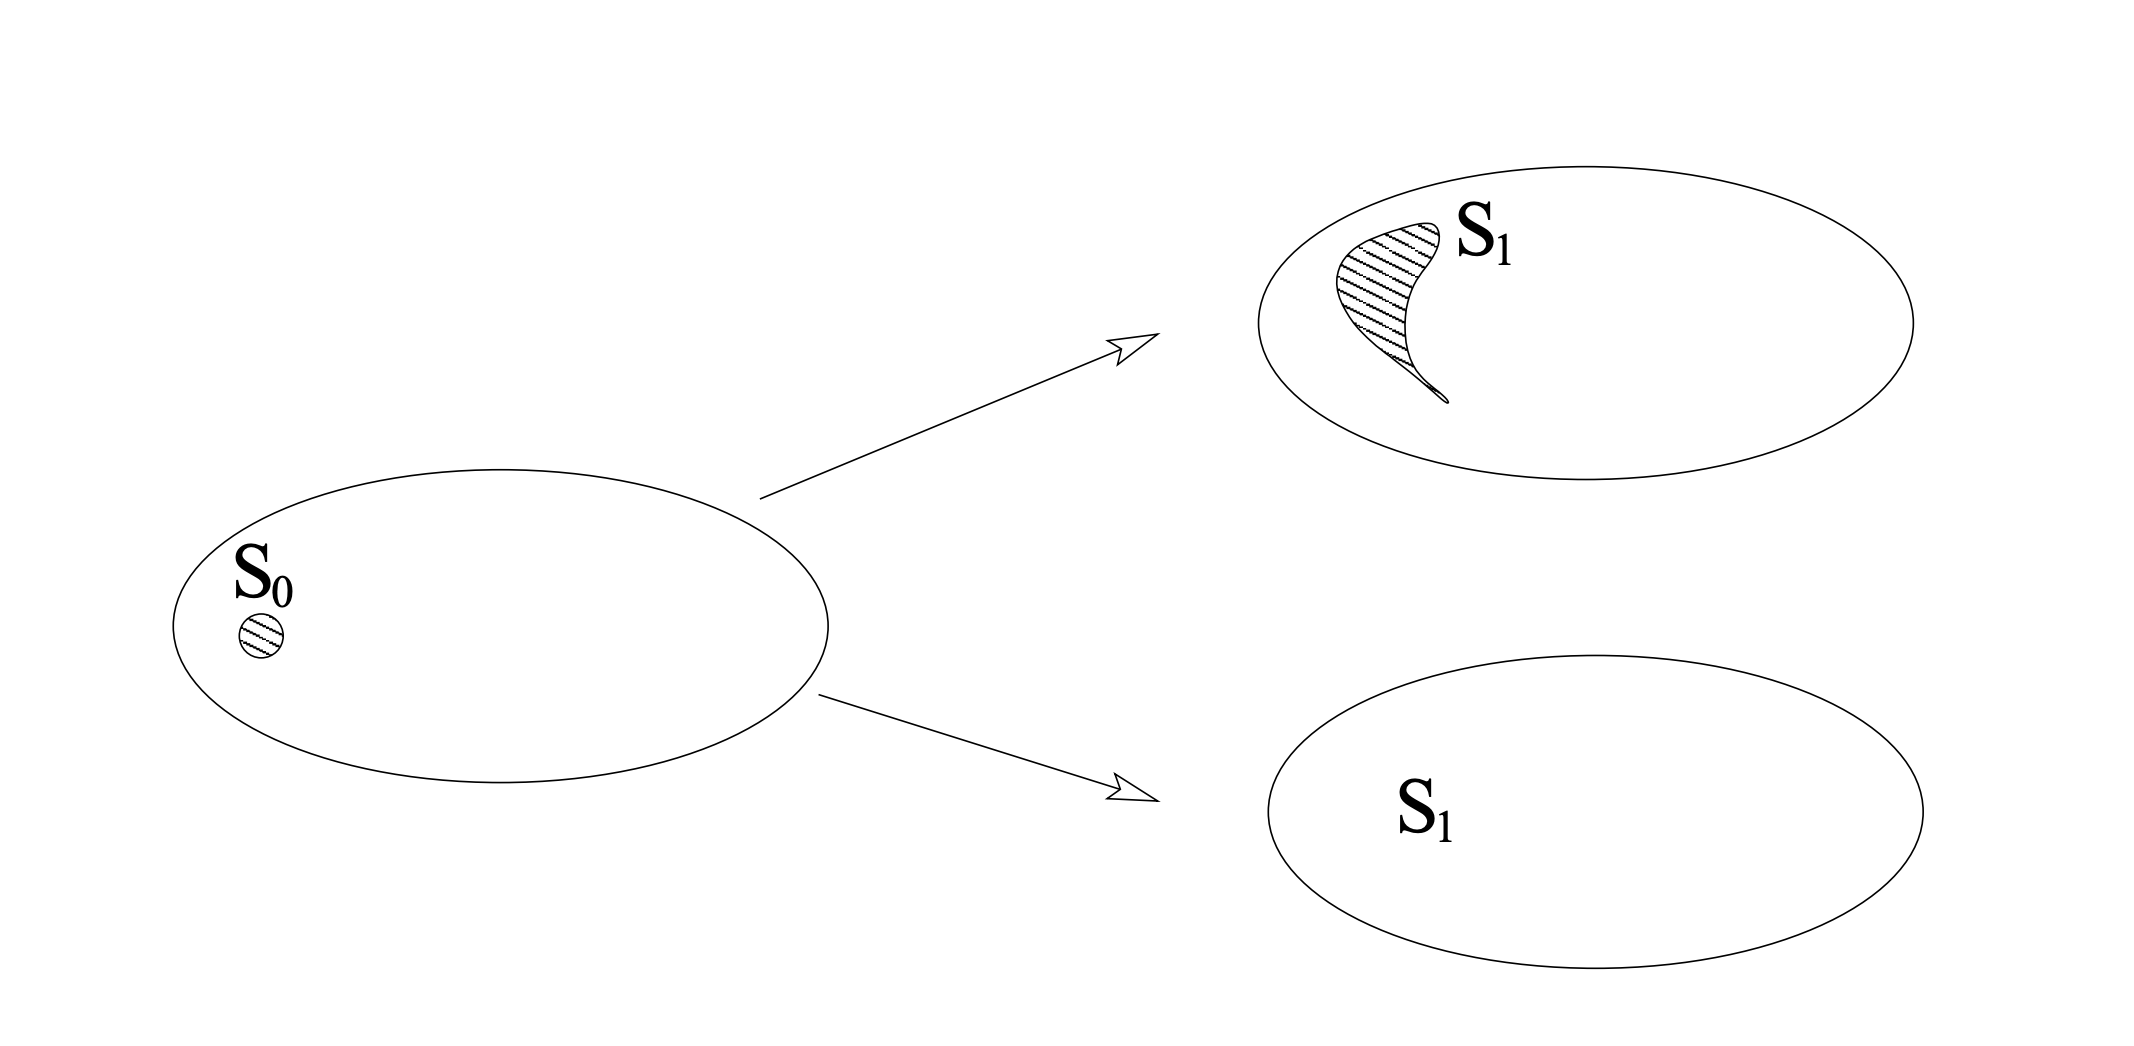
\includegraphics[width=4in]{ESP.png}
  \caption{When \(Z\) is small, the set grows. When \(Z\) is large, the set shrinks. (\cite{ESP})}
  \label{fig:2}
\end{center}
\end{figure}
 
Let the transition kernel of ESP be denoted by \(\mathbf{K}(S, S')\).
 Then the volume-biased ESPs are Markov chains with the following transition kernel:
 \[
   \widehat{\mathbf{K}}(S, S')=\frac{\textrm{vol}(S')}{\textrm{vol}(S)}\cdot \mathbf{K}(S, S').
 \]
As \cite{Shayan} show, volume-biased ESPs can be used to generate a local cluster of vertices around a given seed vertex in time sublinear
in the size of the input graph. 

Now we would like to estimate the likelihood of sequence of vertices generated by the volume-biased ESP.
Since the goal is to learn a latent representation, we introduce a mapping \(\Phi: v\in V\mapsto \mathbb{R}^{|V|\times d}\)
representing the social representation associated with each vertex. Then we wish to maximize
the likelihood
\[
  \mathbb{P}\left[v_i|\Phi(v_1),\ldots, \Phi(v_{i-1})\right].
\]
However, this is often infeasible to compute, so we turn to the language modeling relaxation idea of \cite{Perozzi_2014}.
In terms of vertex representation modeling, this yields us, for some window size \(w\), the following optimization problem:
\[
  \max_{\Phi} \log \mathbb{P}[\{v_{i-w},\ldots, v_{i-1}, v_{i+1},\ldots, v_{i+w}\}|\Phi(v_i)].
\]
Here, instead of using the context to estimate probability of any given vertex, we compute the probability of context given
the vertex. Furthermore, it removes the ordering constraint on the context vertices which allows us to capture the notion of ``nearness''
that is provided by the ESPs. This relaxation idea comes from language modeling
literature: consider the analogous situation where the sequence of vertices can be considered as a sentence and we would like to maximize the
likelihood of a given word over the entire training corpus.

As claimed, the method produces a low dimensional, continuous mapping \(\Phi\) that exploits the
local graph clustering offered by the ESPs. As a result of the relaxation, it also adapts fairly well to
changes in the network. In fact, \cite{Perozzi_2014} provide a streaming algorithm for their truncated
random walks which can easily be modified to fit out purpose.

In the next section, we offer three main algorithms: GenerateSample that simulates the volume-biased ESP (\cite{Shayan}), EvoWalk that generates the
near vertices and SkipGram that performs the language modeling optimization suggested above (\cite{mikolov2013efficient}).
\begin{figure}
  \begin{center}
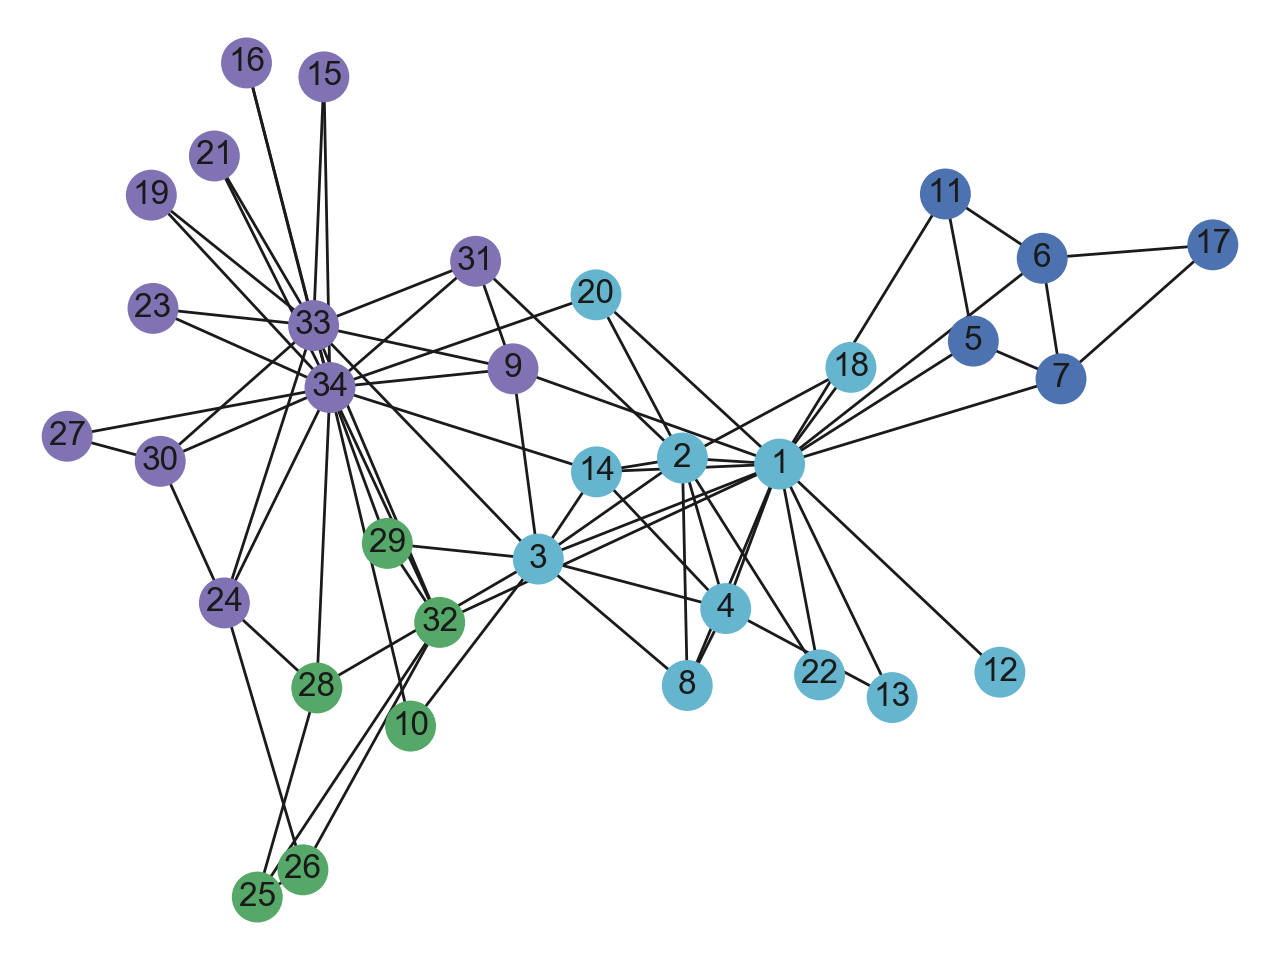
\includegraphics[width=4in]{embd/karate.png}
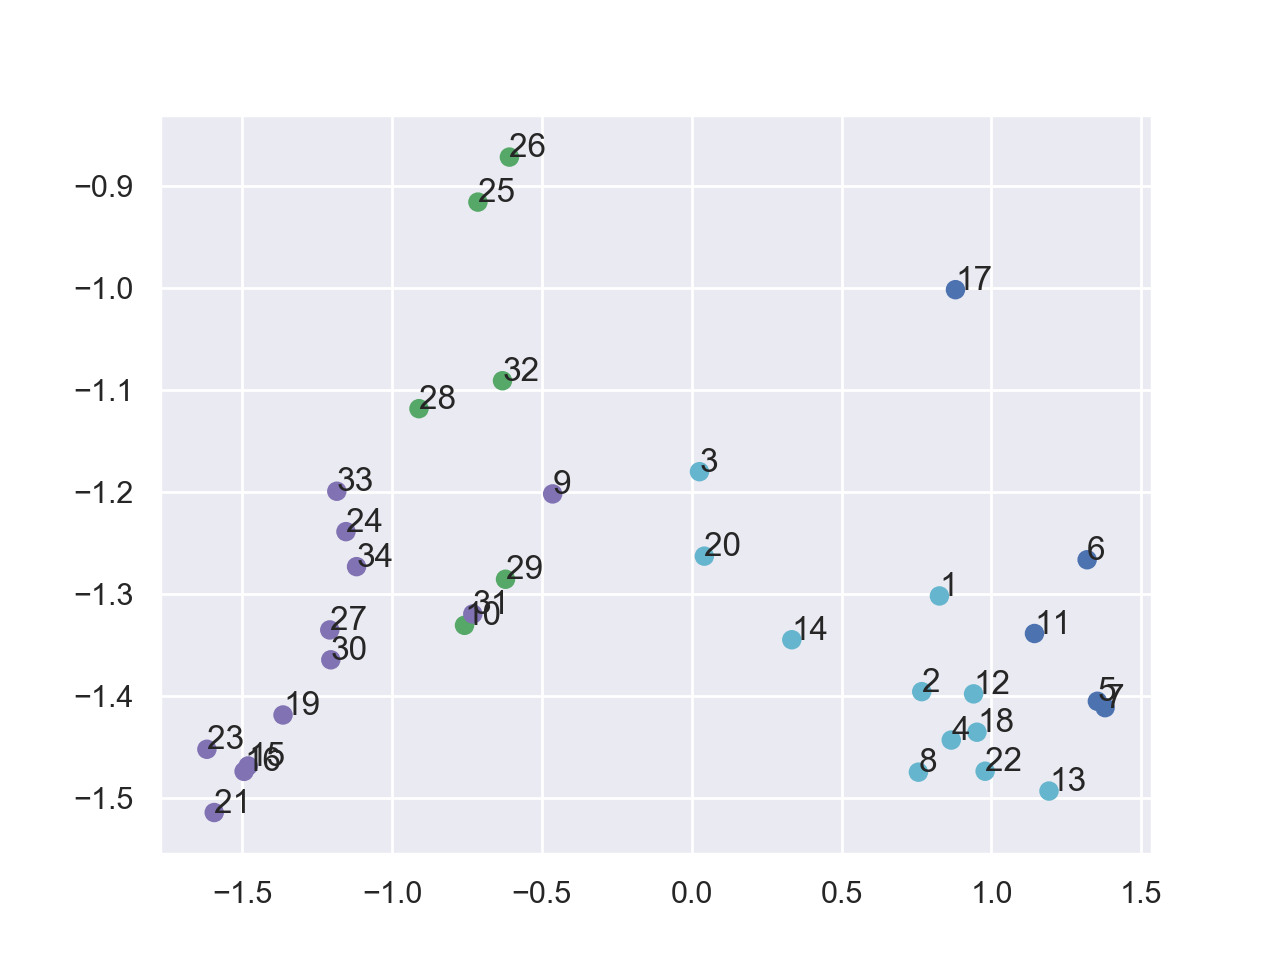
\includegraphics[width=4in]{embd/karate_embd.png}
  \end{center}
\caption{The proposed method learns a continuous embedding of vertices in \(\mathbb{R}^d\)
        that preserves the community structure of vertices in the input graph.
        Top: \cite{Zachary}'s karate graph where the color of vertices represents
        clustering. Bottom: An embedding of the input graph in \(\mathbb{R}^2\).
        Note the strong communal preservation in the embedding.}
  \label{fig:1}
\end{figure}

\newpage
\section{Algorithms}

generate sample ...

\begin{algorithm}
  \caption{EvoWalk(\(G, w, d, \gamma, t\))}
  \SetKwInOut{Input}{Input}
  \SetKwInOut{Output}{Output}
  \Input{graph \(G(V, E)\), window size $w$, embedding dimension $d$,\newline  ESPs per vertex $\gamma$, ESP stopping time $t$.}
  \Output{A matric of vertex representations \(\Phi\in\mathbb{R}^{|V|\times d}\)}
  Initialization: Sample $\Phi$ from $\mathcal{U}^{|V|\times d}$\\
  \For{$j=0\to \gamma$}{
    $\mathcal{O} \leftarrow \textrm{Shuffle}(V)$\\
    \For{$v_i\in\mathcal{O}$}{
      \For{$\phi\in\{0.1, 0.2, \ldots, 1\}$}{
      $k\leftarrow \log\textrm{Vol}(V)$\\
      $\mathcal{W}_{v_i}\leftarrow$ GenerateSample($G, v_i, t, \infty, \phi, k$)\\ \tcp*{ Use EvoPar for result with high probability}
      \If{$\mathcal{W}_{v_i}\neq \emptyset$}{break}
      }
      SkipGram($\Phi, \mathcal{W}_{v_i}, w$)
    }
  }
\end{algorithm}

EvoWalk generates \(\gamma\) ESPs for each vertex with minimal conductance to ensure homophily and relatively low volume to ensure
locality. In order to generate the minimal conductance set, we call GenerateSample with an epsilon net on the
values of \(\phi\in \{0.1, 0.2, \ldots, 1\}\) and break on first instance. Then we perform the relaxed optimization suggested in the previous section for each cluster found
by ESP in EvoWalk. SkipGram is a prevalent algorithm in language modeling literature for this procedure:
\begin{algorithm}
  \caption{SkipGram(\(\Phi, \mathcal{W}_{v_i}, w\))}
  \For{$v_j\in \mathcal{W}_{v_i}$} {
    \For{$u_k\in \mathcal{W}_{v_i}[j-w:j+w]$} {
      $J(\Phi)\leftarrow -\log \mathbb{P}[u_k|\Phi(v_j)]$   \tcp*{Negative log-likelihood}
      $\Phi\leftarrow \Phi -\alpha \cdot \partial_{\Phi} J$  \tcp*{Gradient descent; learning rate \(\alpha\)}
    }
  }
\end{algorithm}

SkipGram (\citet{mikolov2013efficient}) iterates over vertices \(u_k\) in window \(w\) around all vertices \(v_j\) in the
given local cluster \(\mathcal{W}_{v_i}\). For all \(v_j\), we maximize \(\mathbb{P}[u_k|\Phi(v_j)]\)
by performing a gradient descent on its negative log-likelihood. The following theorem provides
an efficient way to calculate \(\mathbb{P}[u_k|\Phi(v_j)]\).

\begin{theorem}
  (Hierarchical Softmax) There exists an algorithm that computes \(\mathbb{P}[u_k|\Phi(v_j)]\) in time \(O(\log |V|)\).
\end{theorem}
\begin{proof}
  Assign the vertices to the leaves of a binary tree. Then if \(b_0, b_1, \ldots, b_{\lceil \log|V|\rceil}\)
  is the path from root to \(u_k\), we have
  \[
      \mathbb{P}[u_k|\Phi(v_j)]=\prod_{l=1}^{\lceil \log|V|\rceil} \mathbb{P}[b_l|\Phi(v_j)],
  \]
  where \(\mathbb{P}[b_l|\Phi(v_j)]\) can be modeled by a binary classifier assigned to the parent of \(b_l\).
  The cost is, therefore, equal to traversal from root to a leaf in a balanced binary tree, and hence, the theorem.
\end{proof}

\section{Empirical Study}

\subsection{Datasets}

\subsection{Results}

\section{Conclusion}

\newpage
\bibliographystyle{plainnat}
\bibliography{final_report}

\end{document}
